
\tikzset{every picture/.style={remember picture}}
\newcommand\myubar[1]{%
\underaccent{\bar}{#1}}


\begin{equation*}
\tikz[baseline]{\node(d4) {$\hat{\myubar{\theta}}_{k+1}$}} = \tikz[baseline]{\node(d5){$\hat{\myubar{\theta}}_{k}$}} + \tikz[baseline]{\node(d6) {$K_{k+1}$}}\tikz[baseline]{\node(d7){$(\underbrace{y_{k+1}-h'_{k+1}\hat{\myubar{\theta}}_{k}})$}}
\end{equation*}
\vspace{1cm}\par
% insert text
\noindent\hfil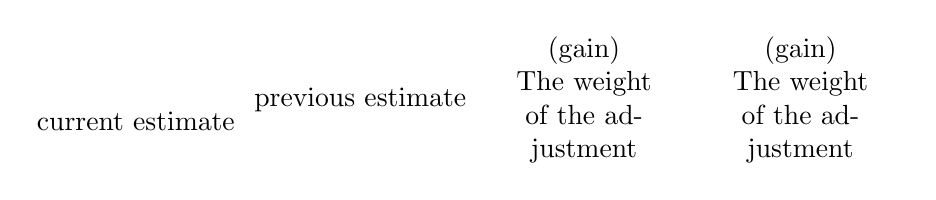
\begin{tikzpicture}
\node (t1) {current estimate};
\node[above right] (t2) at (t1.east) {previous estimate};
\node[right,text width=2.5cm,align=center] (t3) at (t2.east)
 {(gain)\\ The weight\\ of the adjustment};
\node[right,text width=2.5cm,align=center] (t4) at (t3.east)
 {(gain)\\ The~weight\\ of the adjustment};
\end{tikzpicture}
% insert lines between text
\begin{tikzpicture}[overlay]
\draw[blue,thick,->] (d4) to [in=90,out=245] (t1.north);
\draw[blue,thick,->] (d5) to [in=90,out=265] (t2.north);
\draw[blue,thick,->] (d6) to [in=90,out=265] (t3.north);
\draw[blue,thick,->] (d7) to [in=90,out=265] (t4.north);
\end{tikzpicture}

